% LaTeX Notetaking Template for the 2019 Pan-Canadian Self-Organizing Conference on Machine Learning (PC-SOCMLx)
% Template by David Madras, inspired by Meltem Atay's template for the 2018 SOCML

\documentclass{article}
\usepackage[utf8]{inputenc}
\usepackage{enumitem}
\usepackage{dsfont}
\usepackage[margin=3cm]{geometry}
\usepackage{mathtools}
\usepackage{hyperref}
\usepackage{amsfonts}
\usepackage{graphicx}
\usepackage{float}
\title{ARIMA Notes}
\author{Team Fourier}
\date{November 2020}

\begin{document}

\maketitle
\section{Trends}
One commonly encountered time series component is a trend. Trends encompass datasets with non-repetitive generally increasing or decreasing values. An example of a trend is a child's weight as a function of time.
\subsection{Trend Models}
We can model these data by adding a deterministic trend function to white noise:
\begin{equation}\label{1}
X_t=m_t+Z_t
\end{equation}
where $X_t$ is the observation, $m_t$ is the deterministic trend function and $Z_t$ is white noise. Random variables are white noise if they have zero mean and finite variance. This note will cover several methods for fitting \ref{1} to data with trends.
\subsubsection{Linear Regression}
A simple technique would be to perform linear regression on the raw data or a feature augmented data set.
\subsubsection{Simple Moving Average (SMA)}
SMA averages the previous data points with the current sample to reduce noise. For a $2p$-sample moving average, we calculate:
\begin{equation}\label{2}
    \hat{m}_t=\frac{1}{2p+1}\sum_{i=-p}^p m_{t+i} \footnote{Note in financial applications, the averages are taken over the previous $2n+1$ samples rather than $n$ samples on either side of $m_t$}
\end{equation}
where $\hat{m}_t$ is the \emph{simple moving average} of $X_t$. If $m_t$ is linear over $[t-p, t+p]$, then:
\begin{equation}\label{SMA1}
    \hat{m}_t=m_t + \frac{1}{2p+1}\sum_{i=-p}^p Z_{t+i} \approx m_t
\end{equation}
We can generalize SMA as a weighted sum of the samples:
\begin{equation}\label{SMA2}
    \hat{m}_t=\sum_{i=-p}^p \theta_j X_{t+i}
\end{equation}
where $\theta_j$ are the weights. SMA is a special case of this weighted sum with constant weights of $\frac{1}{2p+1}$. The choice of $p$ affects the bias-variance tradeoff, a property of models that determines sensitivity to noise. Read \href{https://www.machinelearningplus.com/machine-learning/bias-variance-tradeoff/}{bias-variance-tradeoff} for more information on this property. Selecting $p$ often requires a hyperparameter search.
\subsubsection{Exponential Moving Average (EMA)}
EMA follows a similar approach to SMA, but instead of constant weights, EMA heavily emphasizes samples closer in time and depends only on previous observations:
\begin{equation}\label{EMA}
    \hat{m}_t=\frac{1-\phi}{\phi} \sum_{i=1}^\infty \phi^i X_{t-i}
\end{equation}
Here the weights $\phi$ remain constant and samples further back in time are exponentially worth less. We multiply the sum by $\frac{1-\phi}{\phi}$ to ensure the weights sum to 1 since $\sum_{i=1}^\infty \phi^i=\frac{\phi}{1-\phi}$.

\subsection{Detrending Data}
To find patterns in trend models, it is often useful to study the stochastic portions of the models. This way we can exploit structure, if any, and create distributions to sample noise for forecasting. One natural approach to obtain the detrended data is differencing:
\begin{equation}\label{differencing}
    \nabla X_t = X_t - X_{t-1} \qquad \forall t \in 2, \ldots, n.
\end{equation}
Let $m_t=at+b$, a linear trend. Then
\begin{align}\label{differencing simplified}
    \nabla X_t &= a(t+1)+b+Z_{t+1}-(at+b+Z_t) \qquad \forall t \in 2, \ldots, n \nonumber \\
    &=a+Z_{t+1}-Z_t.
\end{align}
If $\nabla X_t$ is white noise, we can simply predict $X_{t+1}$ by forecasting $\nabla X_{t+1}$ as the sample mean $\overline{\nabla X}=\sum_{i=2}^n Y_i/(n-1)$. Then, rearranging (\ref{differencing}) we get:
\begin{align}\label{differencing forecast}
    X_{t+1} &= \nabla X_{t+1} + X_t \qquad \forall t \in 2, \ldots, n \nonumber \\
    &= \overline{\nabla X} + X_t.
\end{align}
Similarly, if there are trends after differencing, we can difference again:
\begin{align}\label{differencing quadratic}
    \nabla^2 X_{t} &= \nabla(\nabla X_t) \qquad \forall t \in 3, \ldots, n \nonumber \\
    &= \nabla X_t - \nabla X_{t-1}\nonumber\\
    &= X_t -2X_{t-1}+X_{t-2}.
\end{align}
Second order differencing removes quadratic trends. A nice way to check understanding is to prove why $\nabla^n$ removes $n^{th}$ order trends.

\section{Stationarity}
Stationary processes form the foundation for systematic time series analysis, especially for \textbf{ARMA} (autoregressive moving average) models. There are two standard definitions of stationarity.
\subsection{Strong or Strict Stationarity}
\textit{A stochastic process $\{X_t\}$ is \textbf{strongly stationary} if the joint distribution of any set of samples $(X_{t_1}, X_{t_2}, \ldots, X_{t_k})$ is the same as the joint distribution of $(X_{t_{1}+\tau}, X_{t_{2} + \tau}, \ldots, X_{t_{k}+\tau}) \forall \tau, t_1, \ldots, t_n \in \mathbb{R}$ and $\forall n \in \mathbb{N}$.}\\\\
This allows us to learn summary statistics of the process, such as means and variances. With this knowledge, we can then predict future observations.
\subsection{Weak or Wide-Sense Stationarity}
\textit{A stochastic process $\{X_t\}$ is \textbf{weakly stationary} if
\begin{enumerate}
    \item $\mathbb{E}[X_t]=\mathbb{E}[X_{t+\tau}] \forall \tau \in \mathbb{R}$
    \item $K_{XX}(t, s)=K_{XX}(t+\tau, s+\tau) \forall \tau \in \mathbb{R}$
\end{enumerate}
where $K_{XX}(t, s)$ is the autocovariance function of $X_t$ evaluated at time $t$ and $s$.}\\\\
Strong and weak stationarities do not imply each other. The rest of this note will refer to \emph{weak stationarity} when discussing \emph{stationarity}.
\subsubsection{Autocovariance Function \emph{(acvf)}}
The \emph{acvf} is defined as:
\begin{align}
    K_{XX}(t, s) &= \text{Cov}[X_t, X_s]\nonumber\\
    &= \mathbb{E}[(X_t-\mu_t)(X_s-\mu_s)]\nonumber\\
    &= \mathbb{E}[X_t, X_s]-\mu_1\mu_2\nonumber
\end{align}
From condition 2. we realize that the covariance of two random variables only only depends on $\tau$, the time lag between them. Therefore, we can further simplify the \emph{acvf}:
\begin{equation}\label{acvf}
    K_{XX}(\tau) = K_{XX}(t, t+\tau)
\end{equation}
\subsubsection{Autocorrelation Function \emph{(acf)}}
The \emph{acf} is defined as:
\begin{equation}\label{acf}
    \rho(t, s) = \frac{K_{XX}(t, s)}{\sqrt{\text{Var}(X_t), \text{Var}(X_s}}\nonumber
\end{equation}
which can then be simplified to:
\begin{equation}\label{acf}
    \rho(\tau) = \frac{K_{XX}(\tau)}{K_{XX}(0)}
\end{equation}
\begin{figure}[H]
    \centering
    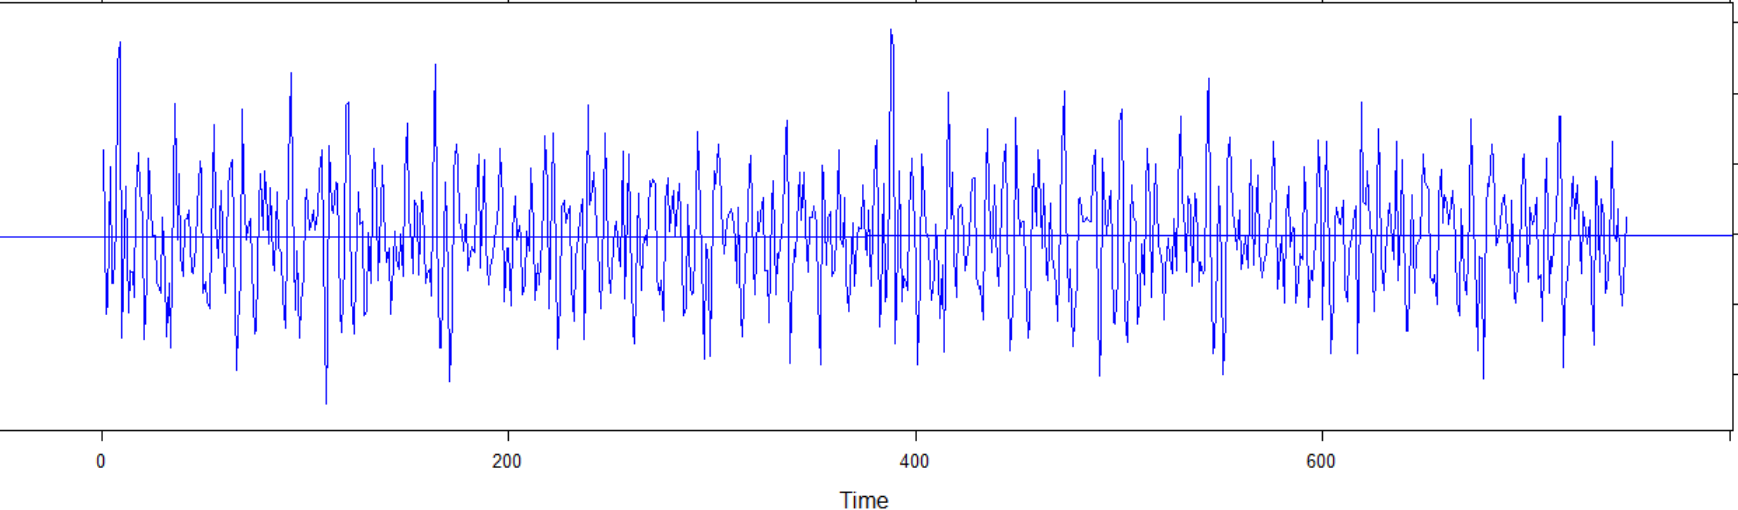
\includegraphics[width=\textwidth]{Stationary.png}
    \caption{Example of stationary process}
    \label{stationary}
\end{figure}
Notice the mean and variance of the data are consistent across time.
\begin{figure}[H]
    \centering
    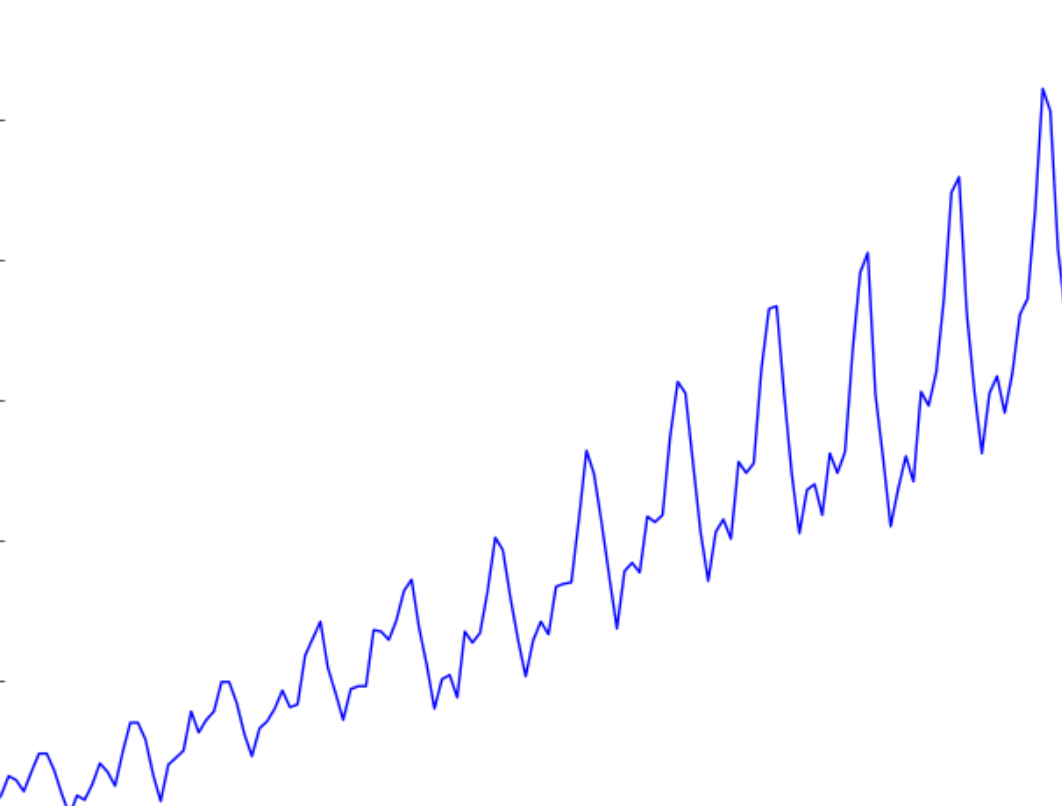
\includegraphics[width=0.5\textwidth]{nonstationary.png}
    \caption{Example of nonstationary process}
    \label{nonstatinoary}
\end{figure}
Notice how both the mean and variance of the sequence increase over time.

\section{Moving Average (MA) Models \protect\footnote{Moving average models are different from the moving average (\emph{SMA}).}}
\textit{Let $Z_t, Z_{t-1}, \ldots, Z_{t-q}$ denote a white noise sequence and $\mu$ denote the mean of the sequence. The textbf{moving average model} of order q, \textbf{MA(q)}, is defined as:
\begin{align}\label{ma model}
    X_t &= \mu + Z_t + \theta_1 Z_{t-1} + \theta_2 Z_{t-2} + \ldots + \theta_q Z_{t-q}\nonumber\\
    &= \mu + \sum_{j=0}^q \theta_j Z_{t-j} \qquad \text{where } \theta_0=1\nonumber\\
    &=  \sum_{j=0}^q \theta_j Z_{t-j}
\end{align}
where $\theta_1, \theta_{2}, \ldots, \theta_{q}$ are the parameters of the model.\\
}
We get (\ref{ma model}) from the second line by remembering the mean of white noise is 0. Moving average models allow for forecasting based on past stochastic terms.
\subsection{Weak Stationarity of an MA(q) Model}
\subsubsection{\emph{ACVF} and \emph{ACF}}
The \emph{acvf} is derived as follows:
\begin{align}\label{ma acvf}
    K_{XX}(\tau) &= \text{cov}(\sum_{j=0}^q \theta_j Z_{t-j}, \sum_{k=0}^q \theta_j Z_{t+\tau-k})\nonumber\\
    &= \sum_{j=0}^q \sum_{k=0}^q \theta_j \theta_k \text{cov}(Z_{t-j}, Z_{t+\tau-k})\nonumber
\end{align}
$K_{XX}(h)$ is only non-zero when $t-j=t+\tau-k$, or when $k=j+\tau$, since $Z_t$ are uncorrelated. We know $k$ is bounded by 0 and $q$ which further means $j$ is bounded by 0 and $q-h$. We can rewrite the \emph{acvf} as:
\begin{equation}\label{ma acvf final}
    K_{XX}(h)=\begin{cases}
        \sigma^2\sum_{j=0}^{q-h} \theta_j \theta_{j+h} \qquad &\text{if } \, h \in 0, 1, \ldots, q\\
        0 \qquad &\text{if } h > q
    \end{cases}
\end{equation}
With some pattern matching, we get the \emph{acf}:
\begin{equation}\label{ma acf}
    K_{XX}(h)=\begin{cases}
        \frac{\sum_{j=0}^{q-h} \theta_j \theta_{j+h}}{\sum_{j=0}^q \theta_j^2} \qquad &\text{if } \, h \in 0, 1, \ldots, q\\
        0 \qquad &\text{if } h > q
    \end{cases}
\end{equation}
Notice that $K_{XX}(\tau)$ is independent of $t$. From this we deduce that:\\
\textit{If \{$X_t$\} follows an MA(q) model, then \{$X_t$\} is \textbf{weakly stationary}.}
\subsubsection{Backshift Operator}
Let $B$ denote the backshift operator. It is defined as:
\begin{align}
    BX_t=X_{t-1}, B^2X_t=X_{t-2}, \ldots, B^nX_t=X_{t-n}\nonumber
\end{align}
and
\begin{align}
    B^{-n}X_t=X_{t+n}, \ldots, B^{-1}X_t=X_{t+1}.\nonumber
\end{align}
\subsubsection{Moving Average Operator}
For parameters $\theta_1, \theta_{2}, \ldots, \theta_{q}$ with $\theta_q \neq 0$, define the \textbf{moving average operator} of order q as:
\begin{equation}\label{moving average operator}
    \theta(B) = 1 + \theta_1 B + \ldots + \theta_q B^q.
\end{equation}
This allows us to succinctly write an MA(q) model from (\ref{ma model}) as:
\begin{equation}
    X_t = \theta(B)Z_t.
\end{equation}
\subsection{Invertibility}
Consider an MA(1) model with acf:
\begin{equation}
    \rho(1)=\frac{\theta}{1 + \theta^2}\nonumber
\end{equation}
For any value of $\theta$, $1/\theta$ gives the same autocorrelation. Therefore, there is no unique solution for the parameters of an MA(1) model. To enforce a unique solution, we impose a theoretical restriction to only consider MA(1) models with $\lvert \theta \rvert < 1$. This condition is called \emph{invertibility}. More broadly, \\
\textit{An MA(q) model $X_t=\theta(B)Z_t$ is invertible iff it can be written as
\begin{align}\label{invertible}
    Z_t&=\pi(B)X_t\nonumber\\
    &= \sum_{j=0}^{\infty} \pi_j X_{t-j}
\end{align}
where $\pi(B)=\sum_{j=0}^{\infty} \pi_j B^j$ and $\sum_{j=0}^{\infty} \lvert \pi_j \rvert < \infty$ and $\pi_0=1$.}

\section{Autoregressive (AR) Models}
\textit{Let $Z_t, Z_{t-1}, \ldots, Z_{t-q}$ denote a white noise sequence and $c$ a constant. The \textbf{autoregressive model} of order p, \textbf{AR(p)}, is defined as:
\begin{align}\label{ar model}
    X_t &= c + Z_t + \phi_1 X_{t-1} + \phi_2 X_{t-2} + \ldots + \phi_p X_{t-p}\nonumber\\
    &= c + Z_t + \sum_{j=0}^p \phi_j X_{t-j} \qquad \text{where } \phi_p \neq 0
\end{align}
where $\phi_1, \ldots, \phi_p$ are parameters of the model.\\
}
Autoregressive models predict future observations directly using past observations.
\subsection{Autoregressive Operator}
For parameters $\phi_1, \ldots, \phi_p$ with $\phi_p \neq 0$, define the \textbf{autoregressive operator} of order p as:
\begin{equation}\label{ar operator}
    \phi(B)=1-\phi_1B-\ldots \phi_p B^p.
\end{equation}
This allows us to write an AR(p) model from (\ref{ar model}) as:
\begin{equation}
    \phi(B)X_t = Z_t
\end{equation}
which has the polynomial form
\begin{equation}\label{ar poly}
    \phi(z)=1-\phi_1z-\ldots \phi_p z^p.
\end{equation}
\subsection{Causality}
Let us take the case of an AR(1) model:
\begin{equation}\label{ar1}
    X_t = Z_t + \phi X_{t-1}\nonumber
\end{equation}
We can rewrite (\ref{ar1}) as:
\begin{align}\label{ar1 soln}
    X_t &= \frac{Z_t}{\phi(B)}\nonumber\\
    &= \frac{1}{1-\phi B} Z_t
\end{align}
Notice we have the sum of a geometric series for $\lvert \phi \rvert < 1$:
\begin{align}
    X_t &= (1 + \phi B + \phi^2 B^2 + \ldots)Z_t\nonumber\\
    &= \sum_{j=0}^{\infty} \phi^j Z_{t-j}
\end{align}
Now consider $\lvert \phi \rvert > 1$. With some clever algebraic manipulation we can get:
\begin{align}\label{ar greater 1}
    X_t &= (-\frac{B^{-1}}{\phi}-\frac{B^{-2}}{\phi^2}-\ldots)Z_t\nonumber\\
    &= -\frac{Z_{t+1}}{\phi} -\frac{Z_{t+2}}{\phi^2}-\ldots\nonumber\\
    &= - \sum_{j=1}^{\infty}\frac{Z_{t+j}}{\phi^j}.
\end{align}
We see for this case that $X_t$ depends on future stochastic values, which usually does not work for forecasting. For an AR(1) model, a unique stationary solution is causal when $\lvert \phi \rvert < 1$ because it only depends on present and past values of $\{Z_t\}$. An AR(1) model with $\lvert \phi \rvert > 1$ is non-causal because it depends on future values. An exercise to ensure understanding is to show why no stationary solution exists for $\lvert \phi \rvert=1$.\\
\textit{We define an AR(p) model as \textbf{causal} if $\phi(z)\neq 0 \text{ for } \lvert z \rvert \leq 1$.}\\
Similar to invertibility for MA(q) models,\\
\textit{An AR(p) model is causal iff it can be written as
\begin{align}\label{causal}
    X_t &=\psi(B)Z_t\nonumber\\
    &= \sum_{j=0}^{\infty}\psi_j Z_{t-j}
\end{align}
where $\psi(B)=\sum_{j=0}^{\infty}\psi_j B^j$ and $\sum_{j=0}^{\infty}\lvert \psi_j \rvert < \infty$ and $\psi_0=1$.}

\subsection{Weak Stationarity of an AR(p) Model}


\section{References}
\url{https://en.wikipedia.org/wiki/White\_noise}\\
\url{https://www.machinelearningplus.com/machine-learning/bias-variance-tradeoff/}\\
\url{https://people.duke.edu/~rnau/411diff.htm}
\end{document}
